\documentclass[12pt]{article}

% Language setting
% Replace `english' with e.g. `pathspanish' to change the document language
\usepackage[english]{babel}

% Set page size and margins
% Replace `letterpaper' with`a4paper' for UK/EU standard size
\usepackage[a4paper,top=2cm,bottom=2cm,left=3cm,right=3cm,marginparwidth=1.75cm]{geometry}

% Useful packages
\usepackage{amsmath}
\usepackage{graphicx}
\usepackage[colorlinks=true, allcolors=black]{hyperref}

\begin{document}

%title
\title{\underline{Project report - AutoPylot}}
\date{March 2022}


\author{%
    \\
    Alexandre Girold\\
    Mickael Bobovitch \\
    Maxime Ellerbach \\
    Maxime Gay \\ \\
    Group: Autonomobile 
    }

\maketitle

\centerline{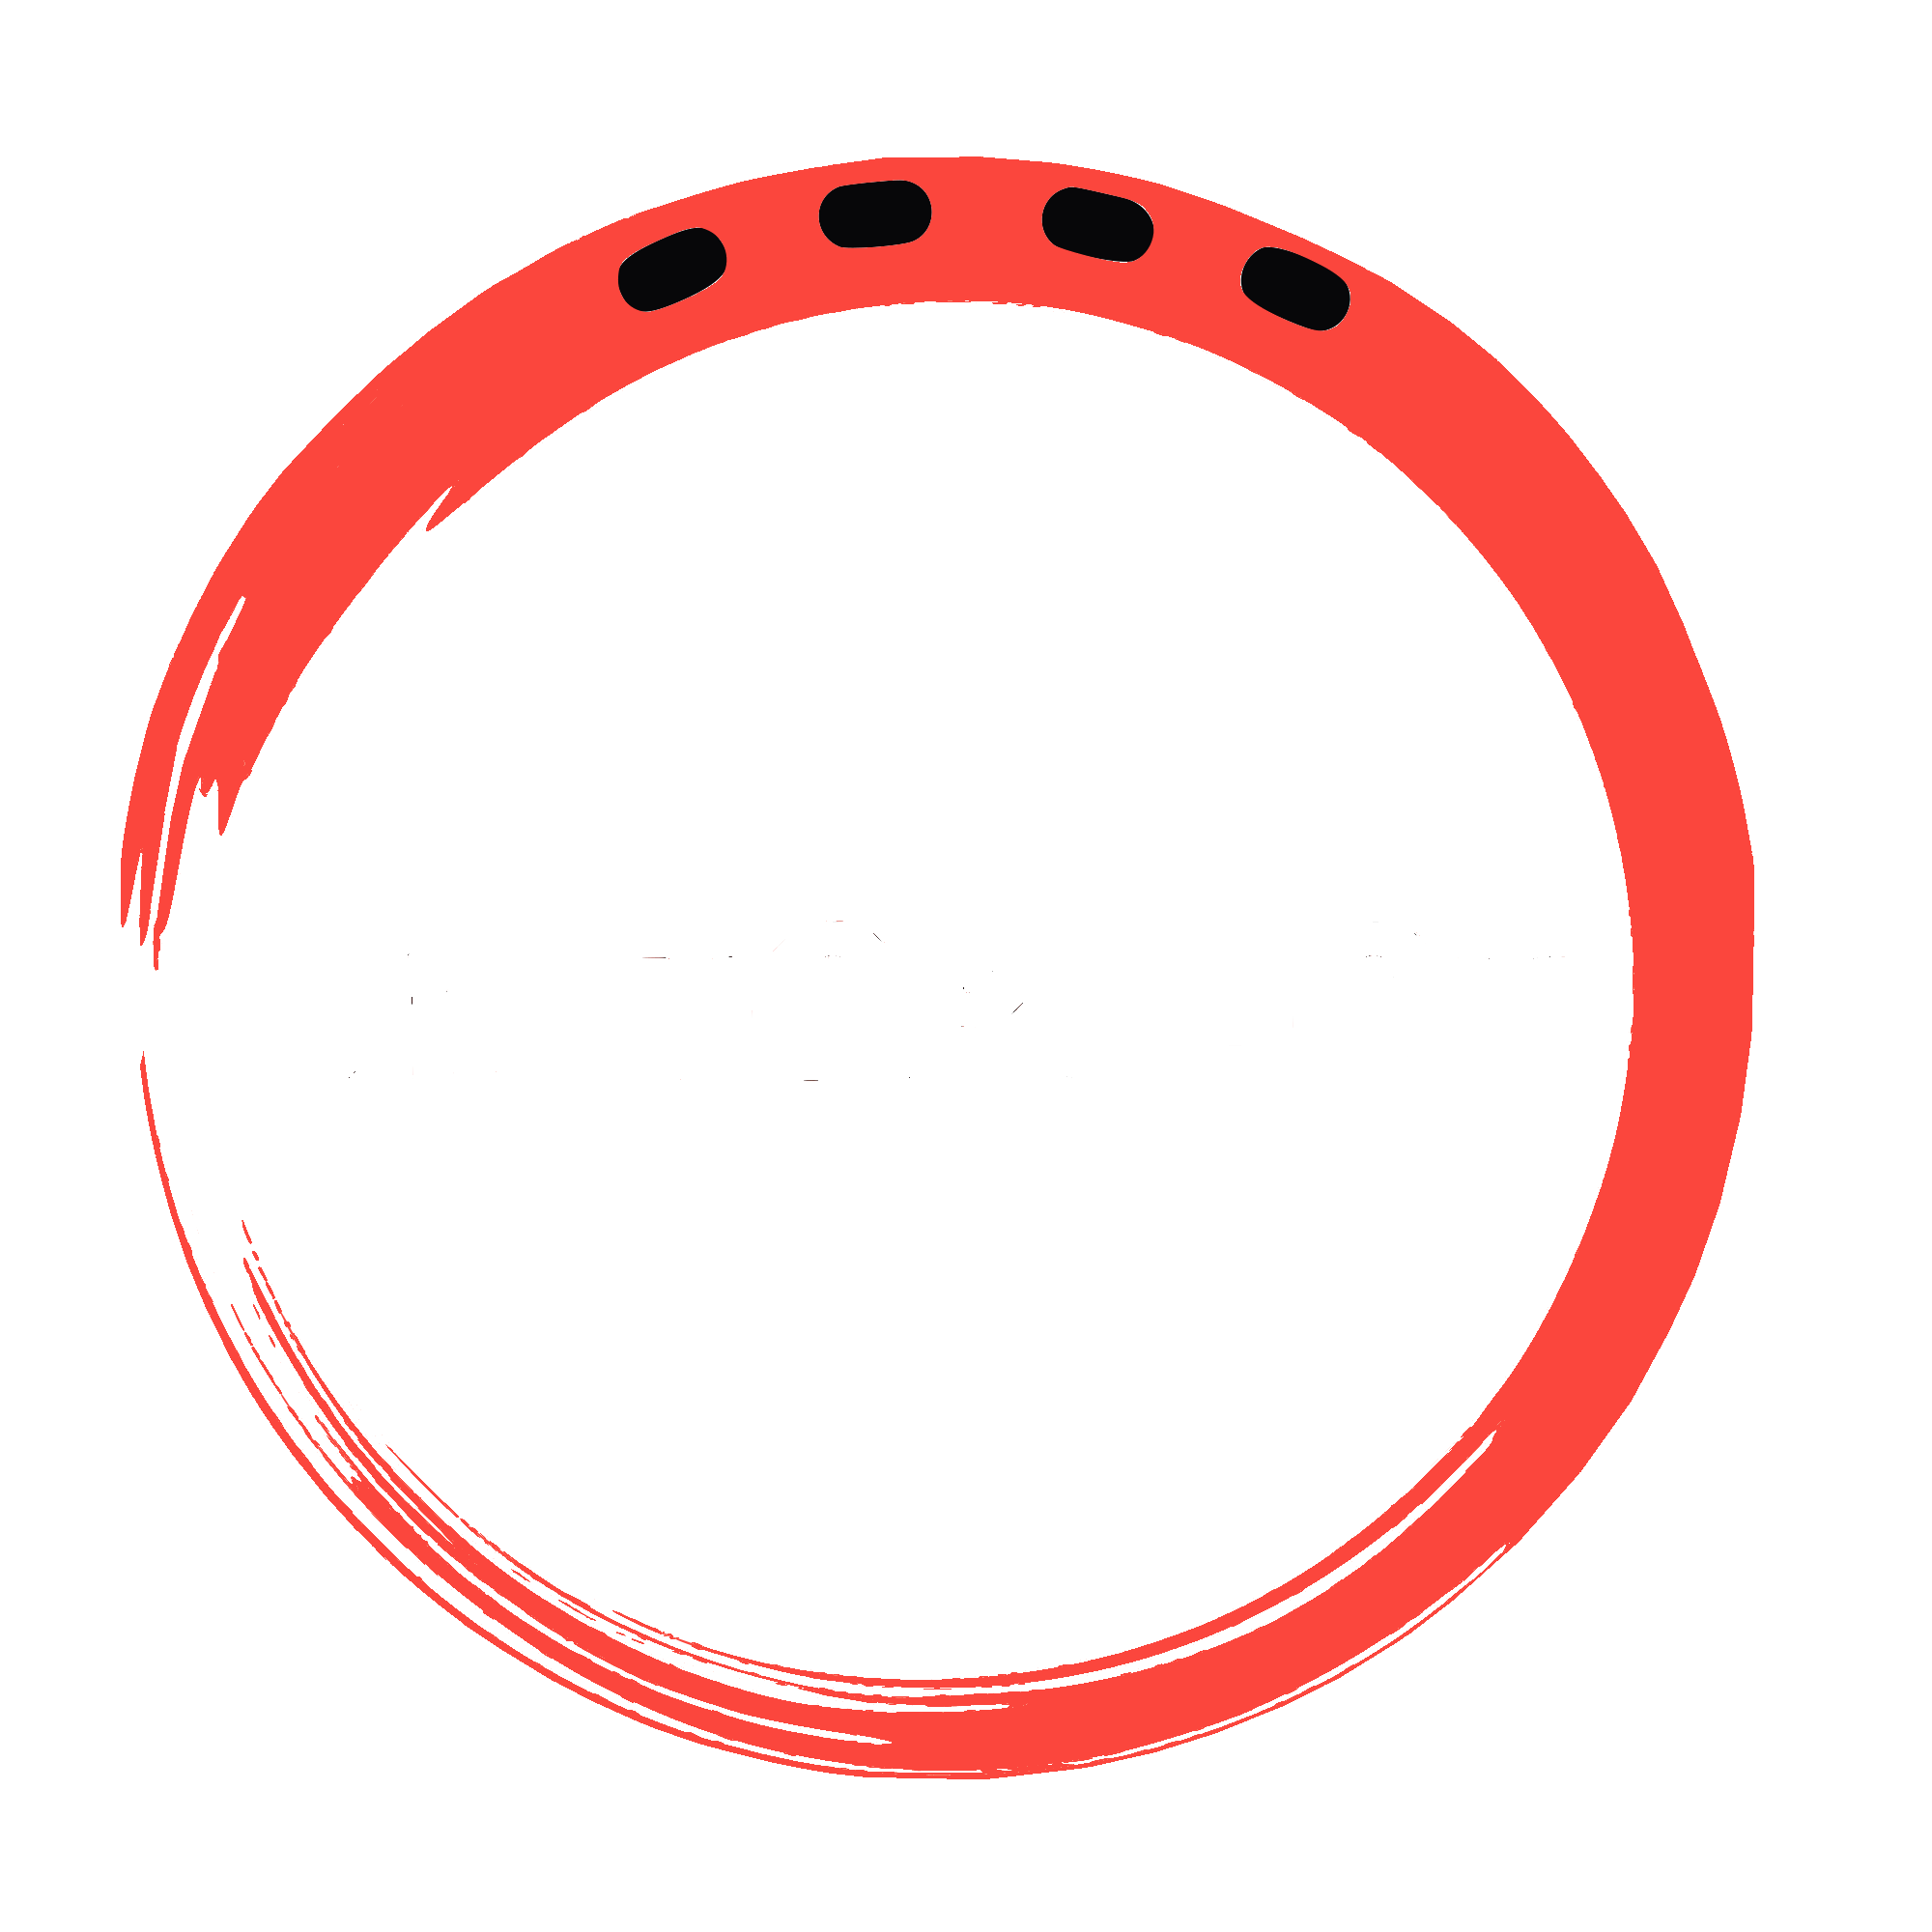
\includegraphics[height=7cm]{../../logos/logo-transparent-white.png}}
\newpage

\tableofcontents
\newpage

\section{Introduction}

\subsection{Project presentation}
Autonomous vehicles and more specifically self driving cars have grasp the attention of many people for good or ill. In this spirit, we have decided with the Autonomobile team to create our first ever project, AutoPylot. The name of our team is of course full of meaning in that regard. Autonomobile is a two-word name, the first one a french word for autonomous : "Autonome", the second one a french word for car : "Automobile". These two-word combined literally mean Autonomous car.\\

What is Autopylot's goal ? 
Drive itself on a track and win races. It may, at first glance seem very simple but not everything is at it seems. Yet we will try to make it as easy to undestand as possible, without omiting crutial information. To achieve our goal, we need to solve many other problems. Those problems can be separate into two distinct groups. \\

The first one would be the software part. Indeed in this project we will need to learn and acquire certain skills, from teamwork to coding in different languages. With those newly acquired skills we will be able to bring machine learning to our car to make it drive itself. This leads use directly to our second part, the more tangible one : hardware. Indeed, as we will progress in our work, we will need to see the results of our work in real life condition. This means implementing our code to a functioning car which will be able to race on a track. \\

This project will lead by a team of four young developers, Maxime Ellerbach, Mickael Bobovitch, Maxime Gay and Alexandre Girold. In this project work will be divided equally amongst all of us, sometimes we will have to work together to achieve our very tight time frame. 

\subsection{Team members}

% Write a small paragraph about yourself, what you like, what you did in the past. Everything is valuable !
\subsubsection{Maxime Ellerbach}
I am a curious and learning hungry person, always happy to learn and collaborate with new people ! Programming, robotics and tinkering has always attracted me. Writting code and then seing the results in real life is something that I find amazing ! I had multiple projects in this field : Lego Mindstorms, a robotic arm, more recently an autonomous car and even a simulator in unity to train even without a circuit at home ! Even if I know quite well the domain of autonomous cars, there is always something new to learn. I look forward working with this team full of hard working people  on such a fun project !

\subsubsection{Mickael Bobovtich}
Roses are red. Violets are blue. Unexpected “Mickael BOBOVITCH “ on line 32. Hello I am a French Student with Russian parents. Lived half of my life in Moscow. Passionate in web dev, servers, and business. Started programming at 13 years old. Created many projects. I like to learn everything, from AI, to UI, from Hardware to Software. Actually I am like OCaml, you need to know me well to appreciate me.

\subsubsection{Maxime Gay}
I am 18 years old,  and I am crazy about investment, finance and especially cryptocurrencies and blockchain. I already worked with a team on different Investment projects and during summer Jobs but this is the first time that I am working on such a  project. Furthermore, I am a beginner in computer Science and autonomous car. However, I am impatient to learn new skills with this incredible team. 

\subsubsection{Alexandre Girold}
I am already getting old. I am 19 years of age, yet I am full of ressources. I am delighted to be able to learn someting new. There are many things which I enjoy from programming to geopolitics. I know this project will push me toward a better me and make great friends along the way. 

\subsection{State of the art}
In this section, we will try to see what was previously made in this sector of industry.
It would not be realistic to compare our 1:10 project to real sized cars such as Tesla's, simply because in a racing environnement,
we don't need to deal with such an amount of safety: pedestrian detection, emergency braking, speed limit detection and other.
So we will only see miniature autonomous racing framework that we would likely race against.\\

The most known is called "DonkeyCar", created by Will Roscoe and Adam Conway in early of 2017. Most of the models trained with DonkeyCar are behavior cloning models, meaning models that tries to replicate the behavior of a driver. This methods uses a big amount of images (input) associated to steering angles and throttle (output), it requires the user to drive the car (collect data) prior to training the model: no examples means no training. The lack of training data often leads to the car leaving the track.\\

One other framework worth looking at is one created by Nvidia called "JetRacer" released in 2019. It uses a different approach from DonkeyCar where the user annotates the images by hand by clicking on where the car should go. The model used is similar to what DonkeyCar uses: a Convolutional Neural Network with one input (the image) and two outputs, one for the steering angle and one for the throttle to apply. \\

Both of those framework are written in python and use packages such as Tensorflow and OpenCV, we will also use them in our project.
\newpage




\section{Realized tasks}

\subsection{Load and save data}

\subsection{Data set}

\subsection{Creation of the logo}

\subsection{Realization of t-shirt}

\subsection{Arduino}

\subsection{Car control}

\subsection{Data vis}

\subsection{Camera}

\subsection{Website}

\subsection{Basic car loop}



% sout : 7 / 03 & 25 / 04 & 06 / 06
\section {Planning}
\subsection {Races}

\begin{tabular}{|l|c|c|c|c|c|c|} 
\hline
Tasks & Race 1 & Race 2 & Race 3 & Race 4 & Race 5 & Race 6  \\ 
\hline
Code controlled motors and servo                & 75\%   & 100\%  &        &        &        &         \\ 
\hline
Drive the car with a controller                 & 25\%   & 100\%   &        &        &        &         \\ 
\hline
Data collection                                 &        & 50\%   & 100\%  &        &        &         \\ 
\hline
Telemetry website                               &        & 25\%   & 100\%  &        &        &         \\ 
\hline
Data processing and augmentation                &        &        & 50\%   & 75\%   & 100\%  &         \\ 
\hline
Basic Convolutional neural network              &        &        & 25\%   & 50\%   & 100\%  &         \\ 
\hline
\begin{tabular}[c]{@{}l@{}}Advanced \\models and optional objectives\end{tabular} &        &        &        &        &        & 50\%    \\
\hline
\end{tabular}

\subsection {Presentations}

\begin{tabular}{|l|c|c|c|} 
\hline
Tasks                                                                             & 1st presentation & 2nd Presentation & Final resentation  \\ 
\hline
Code controlled motors and servo                                                  & 100\%              &                &                    \\ 
\hline
Drive the car with a controller                                                   & 100\%              &                &                    \\ 
\hline
Data collection                                                                   & 75\%               & 100\%          &                    \\ 
\hline
Telemetry website                                                                 & 25\%               & 100\%          &                    \\ 
\hline
Presentation website                                                              & 100\%              & Update         & Update             \\ 
\hline
Data processing and augmentation                                                  &                    & 75\%           & 100\%              \\ 
\hline
Basic Convolutional neural network                                                &                    & 50\%           & 100\%              \\ 
\hline
\begin{tabular}[c]{@{}l@{}}Advanced \\models and optional objectives\end{tabular} &                    &                & 50\%               \\
\hline
\end{tabular}


\section {Task allocation}

\begin{tabular}{|l|c|c|c|c|} 
\hline
Tasks                        & Mickael B. & Maxime G. & Alexandre G. & Maxime E.  \\ 
\hline
Low level car control        &            & x         & x            &            \\ 
\hline
Driving with a controller    &            & x         & x            &            \\ 
\hline
Data storage and handling    & x          & x         & x            & x          \\ 
\hline
Telemetry website            & x          &           &              & x          \\ 
\hline
Presentation website         & x          &           &              & x          \\ 
\hline
Convolutional neural network & x          & x         & x            & x          \\ 
\hline
Main control loop            &            & x         & x            & x          \\
\hline
\end{tabular}

\section {Conclusion}
To sum up, Autonomobile team improved the control of the car with controller, furthermore the data processing is working flawlessly allowing us to load and save images and metadata. Moreover our presentation website is ready, it includes the presentation of the team, some links to download our project and even a road map. Nevertheless, the hardest part is yet to come, indeed we have to work on the AI part of the car and on the telemetry website to have it working by the next project defense. //
The telemtry website is important in order to visualize data to know what is happening inside the car at any moment. We well have to work and learn a lot on this stopic which is really interesting. //

To make a long story short, we spent lot of time on this project, which comport many different sections that are important for the realization of this project and we will do every thing to succed. 


\end{document}
